\setcounter{equation}{0}
%\setcounter{figure}{0}
%\setcounter{table}{0}

\chapter{Experimental details}
%
\section{Overview}

\indent The experiment has been performed in the A2 hall of MAMI facility at the Johannes Gutenberg Universitaet in Mainz, Germany in October 2012 over the course of 21 days.

\indent The key element of the MAMI installation is the Mainzer Mikrotron; it provides a 100\% duty factor electron beam that can be directed to any one of the four experimental halls. The photon beam utilized in the experiment was produced by directing the electron beam onto a thin metallic radiator creating bremsstrahlung radiation. The Glasgow Photon Tagger momentum analyses the recoiling electrons from the bremsstrahlung process and provides information on the energy of the photons. The tagger comprises a large dipole electromagnet and a highly segmented detector apparatus near the focal plane of the magnet. The tin target, located in the center of the Crystal Ball (CB), has been exposed to the bremsstrahlung photon flux and the products of resulting photoreactions have been detected in the CB and TAPS segmented detectors. Since neutral pions have a very short lifetime, order of ~10$^{-18}$s it is not possible to detect them directly. Instead, the products of their dominant decay, two gamma photons, are detected in the apparatus and the pion's 4 momentum is reconstructed from this information. A schematic picture of the MAMI facility is presented In Fig. \ref{a2hallsetup}.

\begin{figure}[H]
\begin{center}
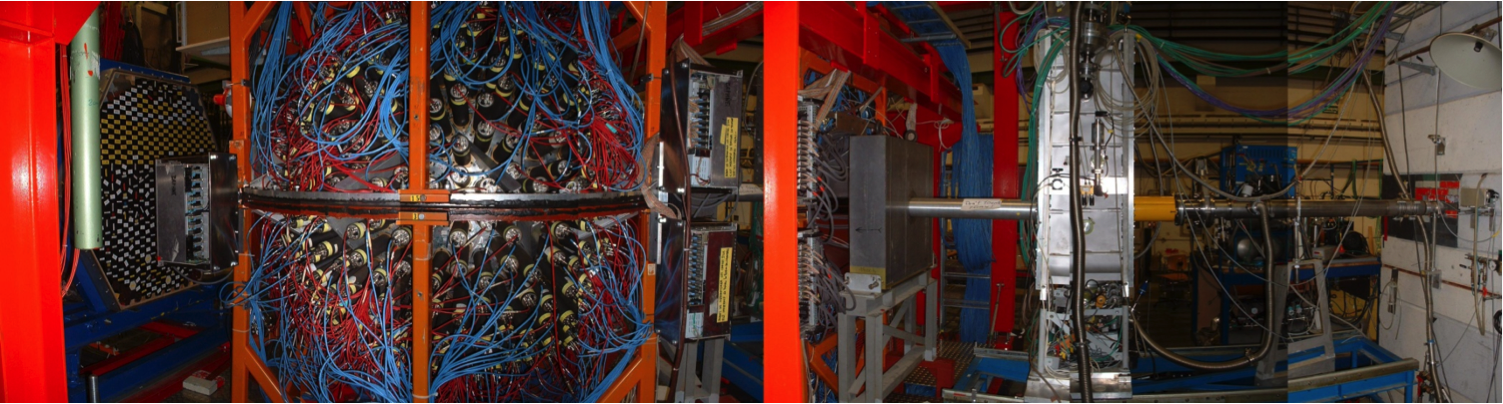
\includegraphics[scale=0.55]{pictures/png/a2hallsetup.png}
\caption{A diagram illustrating the experiential setup in A2 hall at MAMI.}
\label{a2hallsetup}
\end{center}
\end{figure}

In addition to the CB and TAPS detectors, the Edinburgh Particle Identification Detector (PID), providing information about charged particles detected in CB, and Multi Wire Proportional Chambers (MWPC), providing identification of charged particles and tracking information, have been used. The details of all detectors as well as the MAMI facility itself are presented in the following sections.

\section{Mainzer Mikrotron}

\indent The Mainz Microtron (MAMI) is a continuous wave electron accelerator. It is located at the Institut fuer Kernphysik at Johannes Gutenberg Universitaet in Mainz, Germany. MAMI operates since 1979 and in the interim period has been upgraded three times, achieving succesively higher electron beam energies and intensities. The most recent upgrade, to MAMI-C, provides an  electron beam energy up to 1.6GeV with a helicity polarization degree of 80\% and a beam current of over 20$\mu$A (unpolarized electron beams of up to 100uA can be produced).

\indent The MAMI facility operates using a racetrack microtron design.  In this a beam of electrons is accelerated by a series of radio frequency LINAC (linear accelerator) sections and recirculated through the LINACs using a magnetic field. Each time the beam passes through the LINAC its orbit through the magnetic field changes, with higher energy electrons taking wider paths through the magnetic field. These paths are finely tuned such that the electrons always pass through the linac in time with the radiofrequency (rf) electric field frequency applied to the LINACs.  The design of the early stages of the MAMI RTM employ two homogeneous semicircular magnets and a small linear accelerator (LINAC) placed between them (Fig. \ref{microtronplot}).
Repeated passes through LINAC ensure that high beam energy can be achieved even if the acceleration with each pass is relatovely small. The first microtron has been constructed at the National Research Council of Canada in 1947, according to the design of V. I. Veksler, where the electrons, accelerated along circular paths, reached energies of up to 4.6MeV \cite{dehn}. Ever since that first design the idea of a microtron has been worked upon to reach higher electron energies. The concept of a  racetrack microtron (RTM) has been proposed already in 1945 but the first RTM was constructed only in 1961 and provided electron beams of energies up to 12~MeV. 
\begin{figure}[H]
\begin{center}
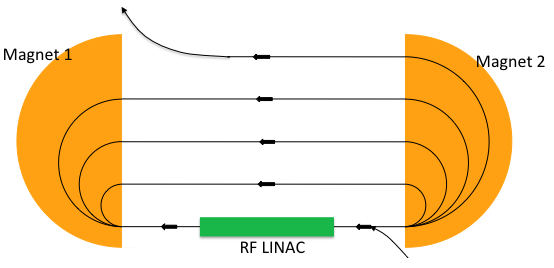
\includegraphics[scale=0.55]{pictures/png/rfm.png}
\caption{Schematics of a simple microtron.}
\label{microtronplot}
\end{center}
\end{figure}

In 1979 a RTM was first used successfully at MAMI facility, producing an electron beam of 14MeV (MAMI-A1). Subsequent upgrade (MAMI-A2) introduced another RTM to the design and allowed for beam energies up to 180MeV in 1983. The need for even higher beam energies inspired yet another upgrade (MAMI B), and in 1990 with the addition of another RTM it was possible to achieve energies of up to 855MeV. However, quickly advancing research in the fields of nuclear and particle physics required even higher energies. The design allowing for beam energies of 1.5GeV however, could not employ another RTM based on the dipole magnet design; the magnets required for achieving such energies would have to weight 2500 tons each which was neither financially nor spatially feasible; for comparison, magnets in the MAMI B design weigh only 450 tons. The issue has been bypassed by adding a harmonic double-sided microtron (HDSM). In this concept, rather than using two magnets bending the beam by 180$^{\circ}$, four 90$^{\circ}$ ets and two accelerating sections have been used (Fig. \ref{mamic}). 

\begin{figure}[H]
\begin{center}
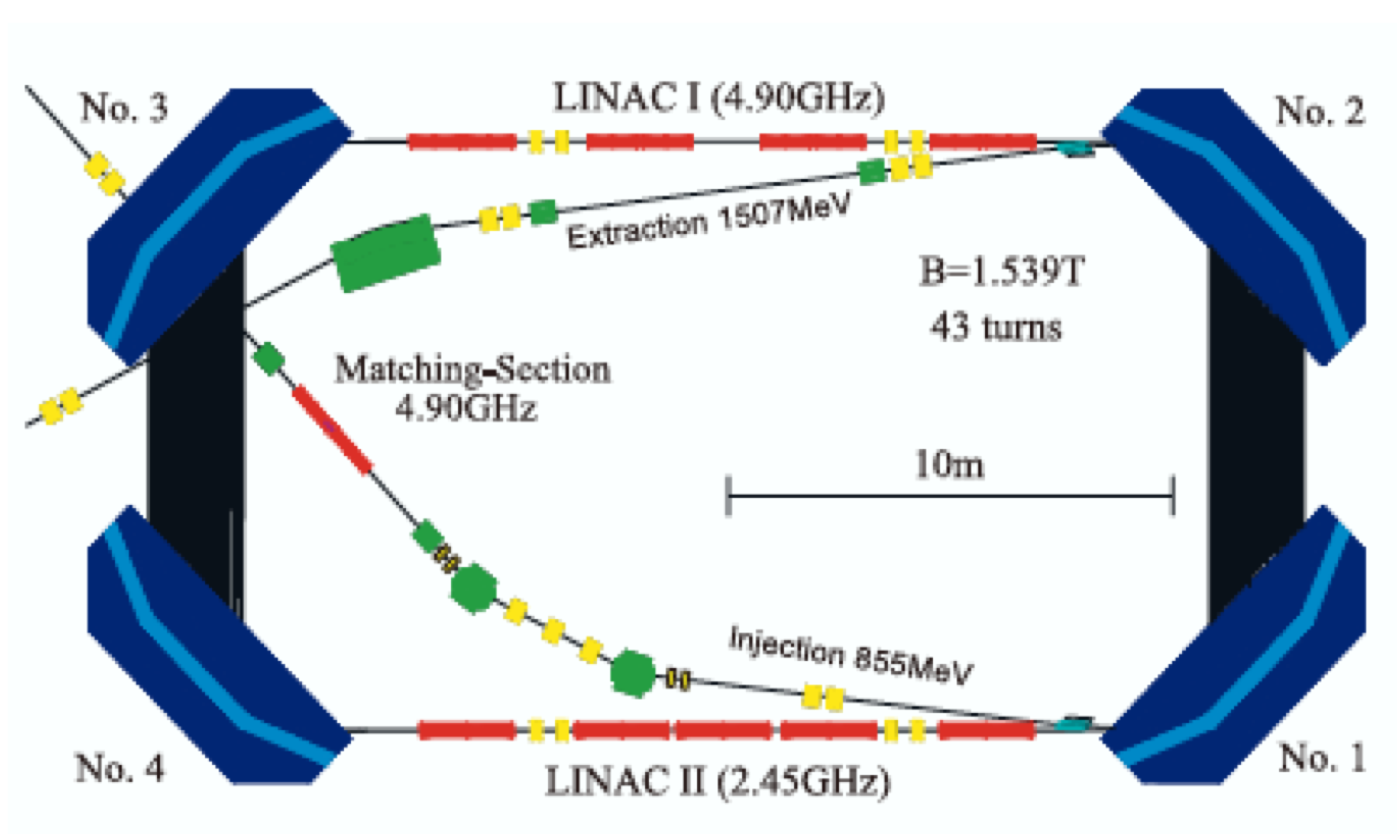
\includegraphics[scale=0.25]{pictures/png/HDSM.png}
\caption{Schematic picture of a harmonic double-sided microtron for MAMI C.}
\label{mamic}
\end{center}
\end{figure}

This design allowed for the production of a 1.508GeV electron beam in December 2006, and energy as high as 1.604GeV has been reached in 2009.

\begin{figure}[H]
\begin{center}
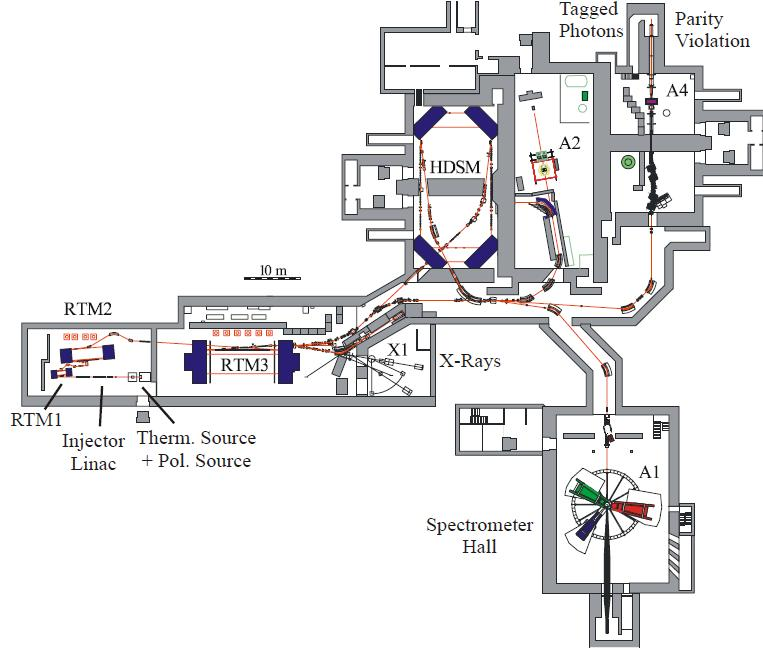
\includegraphics[scale=0.5]{pictures/jpg/mamifloor.jpg}
\caption{Floor plan of the MAMI facility.}
\label{mamifloor}
\end{center}
\end{figure}

\section{Glasgow Photon Tagger}

\indent The experiment has been performed in the A2 hall of MAMI (Fig .\ref{mamifloor}), which houses the installation dedicated to the studies of reactions between high-energy photons with atomic nuclei. The photon beam used in this experiment has been produced when the electrons ejected from RTM3 were directed into A2 hall and incident onto a thin, 10$\mu$m thick, copper radiator. The 855MeV electrons can interact in the electrostatic field of the copper nuclei and radiate photons; the energy of these bremsstrahlung photons can be calculated from:

\begin{equation}
E_{\gamma}=E_{0}-E_{e}
\end{equation}

where $E_{0}$ is the initial beam energy and $E_{e}$ is the energy of the scattered electrons. This equation neglects the energy loss to the recoiling copper nuclei, however, the mass of the copper nucleus is high enough to assume that only negligible amount of kinetic energy has been transferred.

\begin{figure}[H]
\begin{center}
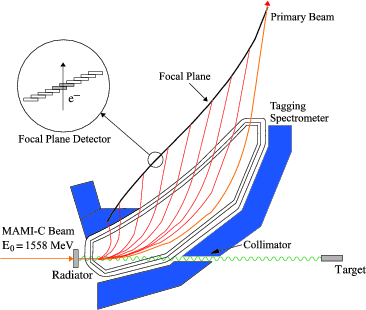
\includegraphics[scale=0.8]{pictures/png/GlaTagger.png}
\caption{Schematic picture of the Glasgow Photon Tagger \cite{marcu}.}
\label{gpt}
\end{center}
\end{figure}

\indent The Glasgow Photon Tagger (GPT) is a large momentum acceptance spectrometer. Electrons, after passing through radiator, first enter the magnetic field of a quadrupole magnet, which focuses them vertically, and then the dipole magnet disperses them horizontally according to their energy. For example, the lower energy electrons associated with the production of higher energy photons are bent more significantly by the field compared to the higher energy electrons. The momentum of the bremsstrahlung electrons is analysed in the Glasgow Photon Tagger (Fig. \ref{gpt}). By identifying the pathe of the electron in the field and correlating the timing of the electron with the subsequet photnuclear reaction in the target then the photons can be characterised event-by-event. This is referred to as a tagged photon beam. Electrons that have radiated bremsstrahlung photons are directed onto a segmented focal plane detector. The electrons that havenÕt radiated any photons follow a curved path into a beam dump.

<<<<<<< HEAD
\indent The focal plane (FP) detector consists of 353 wrapped in a double-sided, aluminized Mylar plastic scintillators \cite{sjhall}. Each of these scintillators is 80mm long and 2mm thick with a varying width of 9-32 mm. The width decreases along the focal plane in order to keep the energy resolution constant. The scintillators overlap by more than half-width (Fig 3.2) what allows for electron detection by coincidence signals in two adjacent detectors with the energy resolution of 2-8MeV, with the average of 4MeV, depending on the beam energy \cite{mcgeorge}; the coincidence condition also allows for significant reduction of the low energy background in the detector.
=======
\indent The focal plane (FP) detector consists of 353 plastic scintillator detectors wrapped in a double-sided, aluminized Mylar \cite{shall}. Each of these scintillators is 80mm long and 2mm thick with a varying width of 9-32 mm. The detector width decreases along the focal plane in order to keep the energy resolution constant. The scintillators overlap by more than a half-width (Fig 3.2) which allows for electron detection by coincident signals in two adjacent detectors. The size of this overlap fixes the achievable energy resolution, which ranges from 2-8MeV with an average of 4MeV, depending on the beam energy \cite{mcgeorge}; the coincidence condition also allows for significant reduction of the low energy background in the detector.
>>>>>>> 05b600032413a648185c176c02b19650e9302a8f

\indent Each scintillator is connected to an R1635 Hamamatsu photomultiplier tube (PMT), which are shielded from the magnetic field by 0.7mm thick steel plates and an individual sheath of $\mu$-metal. The high segmentation of the array allows for the tagging of high-flux photon beams. When used with the 1.508GeV electron beam, the tagger operate at a rate of up to 10$^{8}$ s$^{-1}$ flux photons in the energy range of 0.08-1.401GeV. The maximum rate is determined by the operating limit of the individual PMTs being 1MHz per channel to aviod unnecessary reduction in their operatig lifetime. The bremsstrahlung photons pass the magnetic field of the GPT unaffected and exit into the experimental hall through a channel bored into the dipole magnet.

\indent In order to ensure the small size of the beam spot on the target a 3mm collimator is employed near to the exit of this bored channel. Employing a collimator produces a more well defined beam spot on the target, but also reduces the photon flux.  Without collimation, the photon flux incident upon the target would be related more directly to the number of hits in the FP detector. To determine the exact luminosity of the photon beam, tagging efficiency measurements have to be made where a 100\% efficient lead glass detector is placed in the beamline.  This efficency correction is applied individually to each detector channel in the focal-plane detector, as the efficiency depends on the opening angle of the gamma beam, which dependends on the gamma (or electron) energy. The tagging efficiency is defined as:

\begin{equation}
\epsilon_{tagg}=\frac{N_{\gamma}}{N_{e}}
\end{equation}

\indent where $N_{\gamma}$ is the number of photons passing through the collimator and registered by the lead glass detector, and $N_{e}$ is the number of hits in the FP detector. During the tagging efficiency measurement, carried out as separate runs during the experiment, a lead glass detector is placed in the path of the collimated beam. The beam intensity employed in this measurement is lower than that used in the actual experiment in order to protect the lead glass detector from the potential radiation damage and to reduce the number of multiple hits in the FP detector.

\section{Crystal Ball}

\indent The Crystal Ball (CB) has been constructed and used in various experiments long before  being  installed  at  MAMI.  First  used  in  1970s  for  the  colliding  beam experiments at the SLAC facility to obtain first accurate measurements of $\frac{J}{\psi}$ \cite {oreglia}. Later it has been used at DESY and in Brookhaven National Laboratory and arrived in its current home, the A2 hall at MAMI only in 2002. The CB is a highly segmented calorimeter, it consists of 672 sodium iodide (NaI) crystals, each in a shape of truncated triangular pyramid, and arranged into a shape of a 20 sided polyhedron (Fig. \ref{naigeom}).

\begin{figure}[H]
\begin{center}
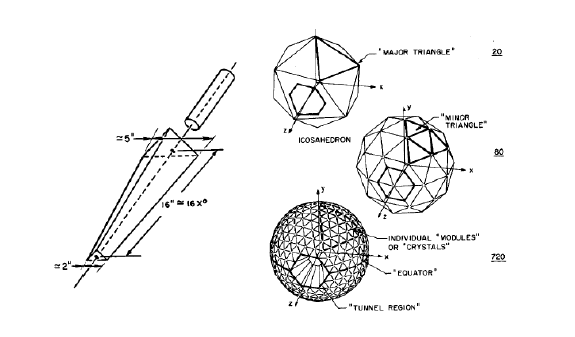
\includegraphics[scale=0.7]{pictures/png/naigeom.png}
\caption{NaI crystal and CB geometry \cite{a2mami}.}
\label{naigeom}
\end{center}
\end{figure}

\indent Having  been  designed  for  the  colliding  beam  experiments,  the  plan  had  to accommodate  the  beamline  running  across  and  through the  center  of  the  CB. Because of that the section corresponding to 24 crystals on opposite poles of the sphere  has  been  cleared  making  room  for  the  beamline  components.  The remaining crystals have been grouped into two, hermetically sealed hemispheres; the isolation of the crystals from the outside environment was essential because NaI is highly hygroscopic and degenerates when exposed to the air moisture.

\indent The outer and inner radii of the CB are 66cm and 25.3cm respectively. The two hemispheres are enclosed within a 1.5mm thick steel casing and the width of the gap between them, the equator region, is 0.8cm thick and consists of two 1.6mm thick steel plates and an adjustable air gap, usually set to 5mm. Such design allows for the coverage close to complete angular range, ~94\% of 4$\pi$.

\indent The of the 20 faces (major triangle) of the CB polyhedron is segmented into 4 smaller triangles (minor triangle)  which  are in turn divided into 9 segments corresponding to individual NaI crystals (Fig. \ref{naigeom}). Each crystal, 40.6cm long with the sides of the inner and outer faces being 5.1cm and 12.7cm respectively, is optically shielded with a reflector paper and aluminized Mylar, and connected to the 5.1cm diameter SRC L50 B01 PMT, chosen for a good linear response over a wide range of energies. These are mounted outside the CB and scintillation light is fed into them through a 5cm air gap and a thick glass window, separating the NaI crystals from the PMTs. This set up constitutes part of the hermetic design helping to maintain isolated environment for the sodium iodide crystals. During the experiment photons produced in the reactions inside the CB trigger an electromagnetic shower which deposits energy in the NaI crystals, chosen for their good energy resolution across a wide range of energies. The amount of deposited energy and the number of crystals hit depend on the reaction studied; the  information  about  the  nature  of  the  particles  detected  in  the  CB  are recovered from the analysis of the hits in the NaI clusters; the basic detection properties  of  the  CB  are  summarized  in  the  below  table \cite {starostin}.
 
\begin{table}[ht]
\caption{Crystal Ball Detection Parameters}
\centering
\begin{tabular}{c c c}
\hline\hline
Energy Photon Resolution & &  \\
 & $\frac{\sigma}{E}$ & ~ $\frac{1.7\%}{E(GeV^{0.4})}$ \\
\hline
Angular Resolution & & \\
 & azimuthal: & ~ $\frac{2^{\circ}}{sin\theta}$ \\
 & polar: & ~2-3$^{\circ}$ \\
\hline
Angular Coverage & & \\
 & azimuthal: & 0 - 360$^{\circ}$ \\
 & polar: & 20 - 160$^{\circ}$ \\
\hline
Time resolution & & \\
 & & $\sigma ~ 2ns$ \\ [1ex]
\hline\hline
\end{tabular}
\label{table_cbparam}
\end{table} 
 

\section{Multi Wire Proportional Chambers}

\indent Inside the tunnel region inside the Crystal Ball another detector by the name of Multi Wire Proportional Chambers (MWPCs) is located. They are tasked with retrieving  information  about  charged particles;  the  design  is that  of  the  one originally used in DAPHNE \cite{audit}.

\indent Each of the two MWPCs is built up of three layers; internal and external stripes acting as cathodes and the middle layer of wires – the anode (Fig. \ref{mwpc}). The cylindrical  cathodes  are  made  from  the  1mm  thick  rohacell  laminated  with aluminum stripes, 4mm wide and  0.1um thick, spaced 0.5mm apart. The stripes are  wound  helically  at  45$^{\circ}$  with  respect  to  the  anode  wires,  in  opposite directions.  The  anode  is  made  up  of  20$\mu$m  Tungsten  wires  2mm  apart  and parallel to the beam direction. The chambers are filled with a gas mixture of argon(79.5\%), ethane (30\%) and freon (0.5\%).

\begin{figure}[H]
\begin{center}
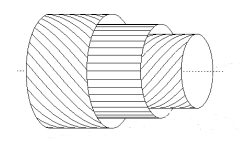
\includegraphics[scale=1.0]{pictures/png/mwpc.png}
\caption{Diagram of MWPC showing the positions of anode wires and cathodes stripes \cite{jalbert}.}
\label{mwpc}
\end{center}
\end{figure}


\indent Correlating  the  hits  in  both  cathode  stripes  and  the  anode  wires  does  the determination of the tracks of charged particles. In the case of neutral particles experiments the information provided by the MWPCs is used to determine the position of the target inside the CB. This information is extracted from the linear fit to the polar angle and z-position of the hits registered in both chambers to obtain the azimuthal and theta and angles for each track. Then the trajectories of multiple tracks are analyzed to find their intersection, and therefore obtain the position of the target. The design of the chambers allows this detector for full 360$\deg$ coverage of the azimuthal angle and the theta range between 21$^{\circ}$ and 159$^{\circ}$; the specifics of the chambers are summarized in the below table.

Table 3.4.1 MWPCs design parameters.

\section{Particle Identification Detector}

\indent The Edinburgh Particle Identification Detector (PID) is located inside the Crystal Ball and surrounded by the MWPCs. It is a $\frac{dE}{dx}$ detector and together with the CB, it provides information about the charged particles.

\indent PID consists of 24 EJ204 plastic scintillators arranged in the cylindrical shape. Each scintillator strip is 500mm long and 4mm thick, and in order to minimize gaps between the adjacent scintillators the design demanded they have right-angle trapezium cross-section. Each strip is wrapped in the aluminized Mylar foil to  optically  isolate  scintillation  light.  The  scintillators  are  connected  to  the Hamamatsu R1635 and E1761-04 PMTs via perspex light guides. An aluminum ring with 24 holes, where the PMTs are positioned so to match the arrangement of  the  scintillator  strips,  supports  the  construction  (Fig. \ref{pid}).  The  entire detector is wrapped in the black Tedlar foil to ensure it is lightproof.

\begin{figure}[H]
\begin{center}
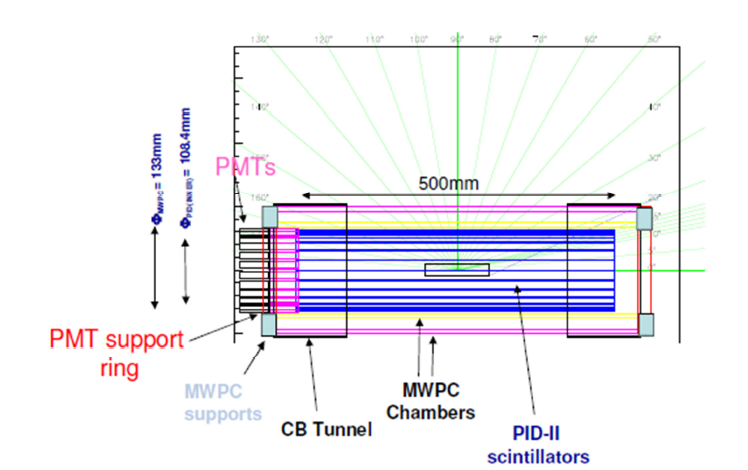
\includegraphics[scale=0.5]{pictures/png/pidschematics.png}
\caption{PID schematics.}
\label{pid}
\end{center}
\end{figure}

<<<<<<< HEAD
\indent The design of allows PID for the full coverage of azimuthal angle and 20$^{\circ}$ to 160$^{\circ}$ coverage of the polar angle, what matches exactly the parameters of the CB. When  a  charged  particle  passes  through  the  scintillator  it  deposits  there  a fraction of its energy and the rest of its energy is detected in the Crystal Ball. The identity  of  such  particle  is  determined  by  correlating  the  events  from  both detectors while enforcing that the hit in the CB is within 15o of the center of the PID scintillator (azimuthal angle). When plotting energy deposited in PID against energy registered in the CB on a two-dimensional plot a characteristic� banana shape is obtained (Fig. \ref{banana}). The proton and pion loci are easily identifiable from such a plot.
=======
\indent The design of allows PID for the full coverage of azimuthal angle and 20$^{\circ}$ to 160$^{\circ}$ coverage of the polar angle, what matches exactly the parameters of the CB. When  a  charged  particle  passes  through  the  scintillator  it  deposits  there  a fraction of its energy and the rest of its energy is detected in the Crystal Ball. The identity  of  such  particle  is  determined  by  correlating  the  events  from  both detectors while enforcing that the hit in the CB is within 15o of the center of the PID scintillator (azimuthal angle). When plotting energy deposited in PID against energy registered in the CB on a two-dimensional plot a characteristicâ banana shape is obtained (Fig. \ref{banana}). The proton and pion loci are easily identifiable from such a plot.
>>>>>>> 05b600032413a648185c176c02b19650e9302a8f

\begin{figure}[H]
\begin{center}
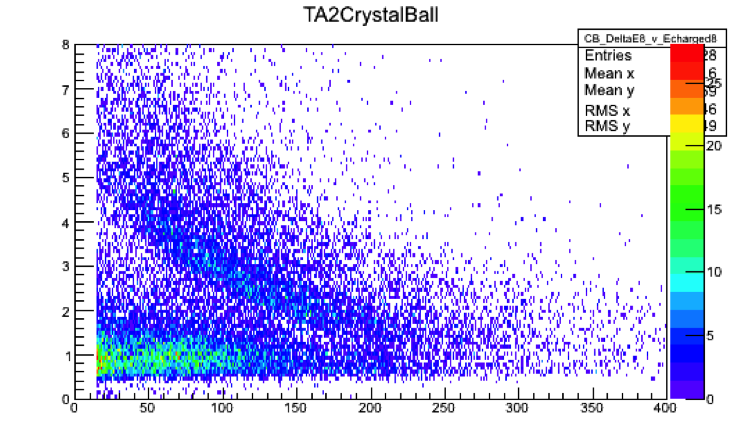
\includegraphics[scale=0.8]{pictures/png/banana.png}
\caption{$\Delta$E-E plots of PID and CB energy deposits.}
\label{banana}
\end{center}
\end{figure}

\section{TAPS}

\indent Because Crystal Ball has been designed for the colliding beam experiments the detector  doesn’t  cover  20o  polar  angle  range  in  backward  and  forward directions, another detector had to be added to the system to make up for it. In MAMI,  the  CB  is  used  for  the  fixed  target  experiments,  where  the  reaction products are Lorentz boosted forward, and because of that an additional TAPS detector  covering  those  missing  forward  20  degrees has  been  mounted \cite{novotny}.

\indent TAPS is located 1.5m downstream from the reaction vertex. It is a segmented calorimeter detector made from 385 hexagonal BaF2 crystals (Fig. \ref{taps}). Each crystal is  25cm long,  wrapped in  8  layers  of 38um thick  UV-reflecting PTFE (Teflon) foil and a single layer of 15um thick aluminum foil for light proofing. The cylindrical end part of each crystal is connected to the Hamamatsu R2059 PMT with silicone glue.

\indent The barium fluoride crystals, even though have much lower scintillation output than NaI crystals used in CB, they have higher density (4.89g/cm3) and larger atomic number, and therefore provide just as good detection efficiency. The most important deciding factor for choosing BaF2 crystals over other materials is its fast timing resolution (~0.6ns), which makes the detector ideal for identifying particles via time of flight (TOF) methods \cite{novotny}.


\begin{figure}[H]
\begin{center}
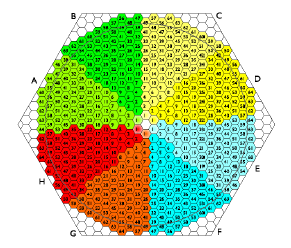
\includegraphics[scale=1.4]{pictures/png/taps.png}
\caption{Diagram of the BaF2 crystals arrangement in TAPS. Different colours represent sectors that can be defined in the trigger if required.}
\label{taps}
\end{center}
\end{figure} 

\indent Directly  in  front  of  TAPS,  there  is  an  array  of  5mm  thick  NE102A  plastic scintillators – the TAPS Veto detector. The output from this detector is collected by the optic fibers in Valvo XP2972 phototubes. This addition to TAPS allows for distinguishing neutral and charged particles by correlating events from TAPS Veto and TAPS, and therefore makes the charged particles identification via $\Delta$E-E technique possible.

\indent Another method used by TAPS to identify particles is time of flight technique. By measuring  the  time  a  particle  traveled  from  the  target  to  TAPS  allows  for distinguishing between slower protons and neutrons and particles traveling at or almost at the speed of light like photons and electrons.

\indent A different method of particle identification, the pulse shape analysis, exploits the fact  that  BaF2  crystals  have  fast  (~0.6ns)  and  slow  (~620ns)  decaying components. Each particle type leaves its own particular imprint on slow and fast components and by comparing the ratios of energy deposited in both, it is possible to tell different particles apart.

\section{Targets}

\indent A previously performed experiment of the coherent $\pi^{0}$ photoproduction on $^{208}$Pb target confirmed the existence of the neutron skin. However, in order to confirm the conclusions of that measurement it was desirable to repeat the experiment for  another  heavy  nuclei.  Furthermore,  it  has  been shown  that  repeated measurements  along  isotopic  chain  promise  better  results  to  put  tighter constraints on the parameters of the neutron rich matter equation of state \cite{centelles}.

\indent The targets used in this experiment were three isotopes of tin ($^{116}$Sn, $^{120}$Sn and $^{124}$Sn); chosen because of its stability, and the elements' easy of availability. Theoretical  calculations  predict  a change of  ~0.05  to  0.15fm  in  the neutron  skin thickness when going across the isotopic chain of tin from $^{116}$Sn to $^{124}$ (Fig. \ref{isochain}) \cite{liewen}. Measuring the skin thickness across the  isotopic  chain  cancels  out  any systematic error,  and  therefore,  allows  to accurately measure the changes predicted by the models.


\begin{figure}[H]
\begin{center}
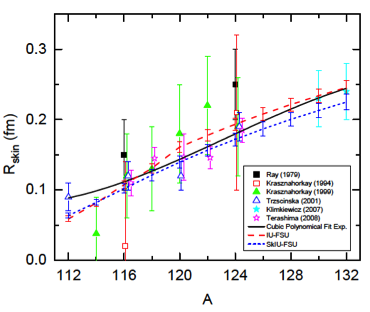
\includegraphics[scale=0.8]{pictures/png/tiniso.png}
\caption{Predictions of neutron skin thickness for tin isotopes from the IU-FSU and SkIU-FSU models.}
\label{isochain}
\end{center}
\end{figure} 

\indent The targets were secured in a target holder by tape and placed inside a PVC tube at the centre of detectors. The details of the targets are given in the below table.

//Table 3.7 Tin targets. - will add later when I find where it is T.T 

\section{Data Acquisition}

\indent The analogue output signal of the detectors' PMTS has been read out and translated into a digital signal by the data acquisition system (DAQ) with the use of charge to digital converters (QDCs), analogue to digital converters (ADCs) and time to digital converters (TDCs). The latter measures the time difference between the start signal of an experimental trigger and the stop signal from a given detector element, thus provided the information about the time of the event. The ADCs give digital information proportional to the pulse height of the signal, while QDCs return digital signal proportional to charge; both these values, pulse height and charge are proportional to the energy deposited in the detector element.

\subsection{Tagger Electronics}

\indent The energy of the bremsstrahlung photons was obtained from the hit position of the recoiling electron on the tagger focal plane. The timing of such hit was used to match the events in the detectors with the hits on the focal plane. Providing that the a signal from the focal plane passed the threshold of the discriminator, a logic pulse was fed to a Compass Accumulation, Transfer and Control Hardware (CATCH) TDC (section 3.8.2) to record the time of the hit. Simultaneously, a signal from the discriminator was sent to FASTBUS scalers, which provided the count rate for each FP detector element. This was subsequently used to determine the photon flux.

\subsection{Crystal Ball Electronics}

\indent As depicted in (Fig. \ref{cbelectronics}), signals from each PMT are sent to fan-out units splitting the analogue output into three signals. One passes to a Flash ADC (F-ADC) via a delay, second goes through the discriminator and branches to a scalar and CATCH TDS. And the third signal is fed to the triggering electronics.

\begin{figure}[H]
\begin{center}
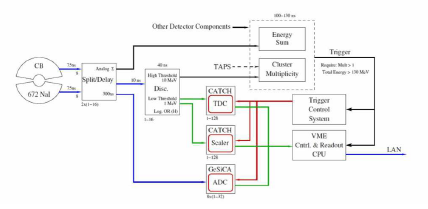
\includegraphics[scale=1.0]{pictures/png/cbelectronics.png}
\caption{Crystal Ball electronics \cite{krambrich}.}
\label{cbelectronics}
\end{center}
\end{figure}

\indent The integral of the pulse from each PMT was obtained from the F-ADCs, which sampled the shape of the signal with a frequency of 40 MHz. Since the DAQ was not prepared to handle such large volumes of data, only the integrals of pulses over three regions were taken. The integration is done over a time window of 750ns (30 signals). The first window was set to sample the pedestal whose signal is a convolution of remnant light and residual charge in the PMTs. The second window was set over the signal, and the third was set to evaluate the tail of the pulse. This set up allowed for the simultaneous measurement of the signal and the pedestal for every event, and with the dynamic subtraction of the pedestal from the signal, the energy resolution of the crystals could have been significantly improved.

\indent Contrary to the typical TDCs, which are started by a hit in a relevant detector and stopped by a logic pulse from the trigger, CATCH TDCs, developed for the Compass experiment at CERN, allow for multiple hits in TDCs \cite{gbruan}. Using a ~10GHz oscillator each TDC is running independently while the CERN-standard trigger control system synchronizes the signals in those TDCs. One of the TDCs is designated as a reference element and attached to the trigger. When an event passes the trigger threshold a logic pulse is sent to this reference TDC and the oscillator value is stored. When other TDCs record a hit, corresponding oscillator value is stored in a buffer. In order to extract the information on the timing of an event the oscillator value stored in the reference TDC has to be subtracted from the oscillator values recorded by other TDCs, the conversion rate of 117 ps/channel is then used \cite{lschmitt}.

\subsection{TAPS Electronics}

\indent The signals from theTAPSPMTs received similar treatment to those from Crystal Ball and were also split into three separate signals. One signal was directed to a TDC via a constant fraction discriminator (CFD), which analyzed the shape of the pulseand provided accurate timing information for the QDCs. The other two signals werefed to separate QDCs, one with integration time of 40ps, other with 200ps, this doubleintegration allows for a pulse shape analysis.

\subsection{Triggering Electronics}

\indent While theevent is being registered by DAQ, no other even is being recorded; this is defined as dead time. In order to reduce theeffects of thedead time, a series of triggers were set up to limit theevents read by DAQ only to those relevant to theexperiment. Two LeCroy LRS 4805 logic units were used to define theconditions an event must satisfy in order to be recorded.

\indent The first level trigger for this experiment required the sum of energy deposited in all 672 NaI crystals to be greater than 40MeV. For the second level trigger, DAQ grouped NAI crystal into clusters of 16, and it was required that there were two hit clusters detected in the CB. When those two conditions were satisfied DAQ read the event and reset the electronics.


\section{Analysis code}

\indent Online analysis and monitoring of the data have been done using the AcquRoot framework. AcquRoot has been written in C++ specifically for the data analysis at MAMI, it uses libriaries and tools of R00T \cite{john, root}. AcquRoot consists of three components, AcquDAQ Data Acquisition, AcquRoot Analysis and AcquMC Event Generator.

\indent Offline analysis was done with a2GoAT (Generation of Analysis Trees). In this framework AcquRoot is used to produce analysis trees containing only basic track information. GoAT software package is used to process those trees; here particle reconstruction, all the data checks and sorting is performed.
